\documentclass{beamer}
\beamerdefaultoverlayspecification{<+->}

% system inspired by the human brain. They consider examples, without task specific programming, e.g. in image recognition, they analyze pics of cats by looking at images that have been labeled as cat or no cat. Collection of units (neurons) that transmit signals from one to another. Each neuron processes signal
% allows computer to learn from observational data

\usetheme{metropolis}      % Use metropolis theme

\usepackage{graphicx}

\title{Neural Networks for Image Classification}
\date{\today}
\author{Catalina Vajiac}
\institute{Saint Mary's College}

\begin{document}
  \maketitle

  \section{Introduction}
  \begin{frame}{Overview}
    \begin{itemize}
      \item Motivation for neural networks
      \item Image classification
      \item PADs project
      \item Workflow
    \end{itemize}
  \end{frame}

  \section{Neural Networks}
  \begin{frame}{What is a Neural Network?}
    \begin{itemize}
      \item loosely inspired by the human brain
      \item collection of units (neurons) that transmit signals to one another
      \item each unit processes signal, propogates forward
      \item allows computer to learn from observational data
    \end{itemize}
    \begin{center}
      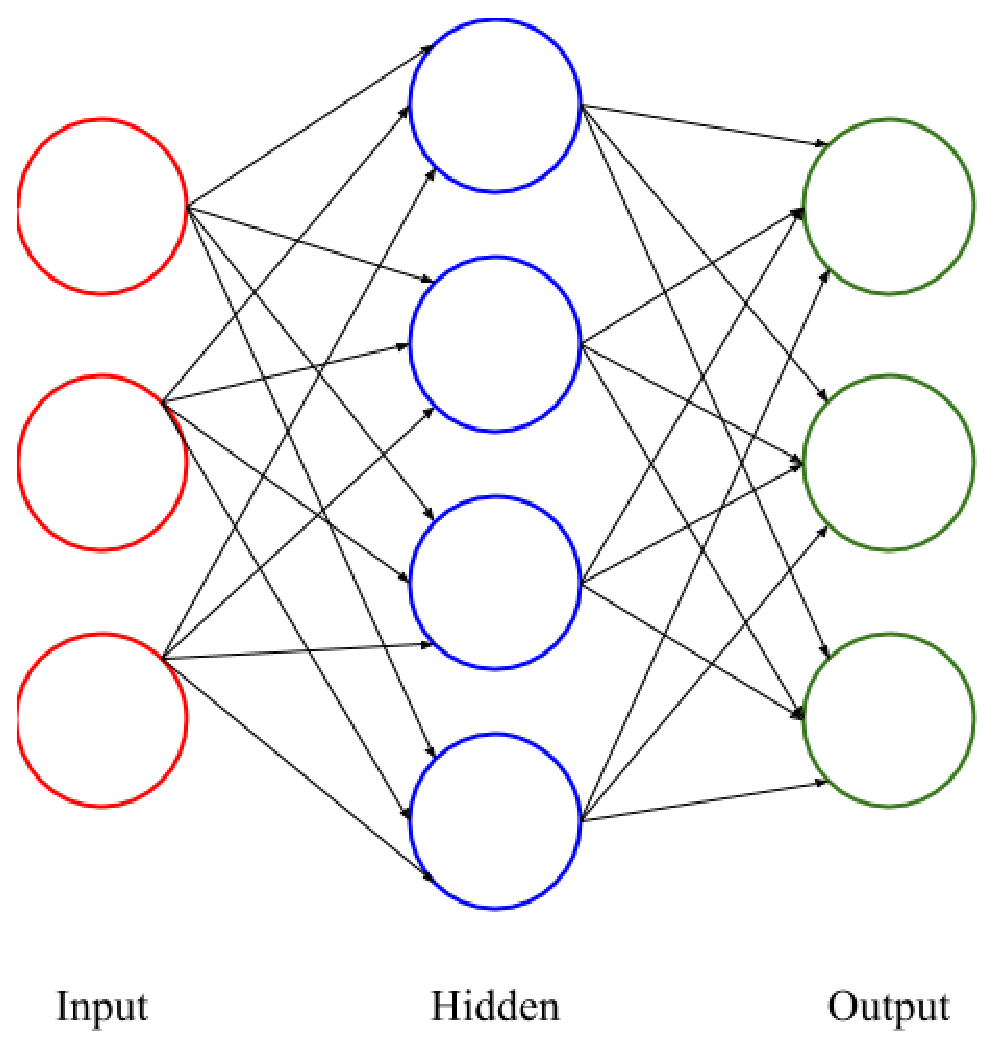
\includegraphics[height=2in]{../figures/neural_network.eps}
    \end{center}
  \end{frame}

  \section{Image Classification}
  \begin{frame}{Goal: Image Classification}
     What is in this image?\\
    \begin{center}
      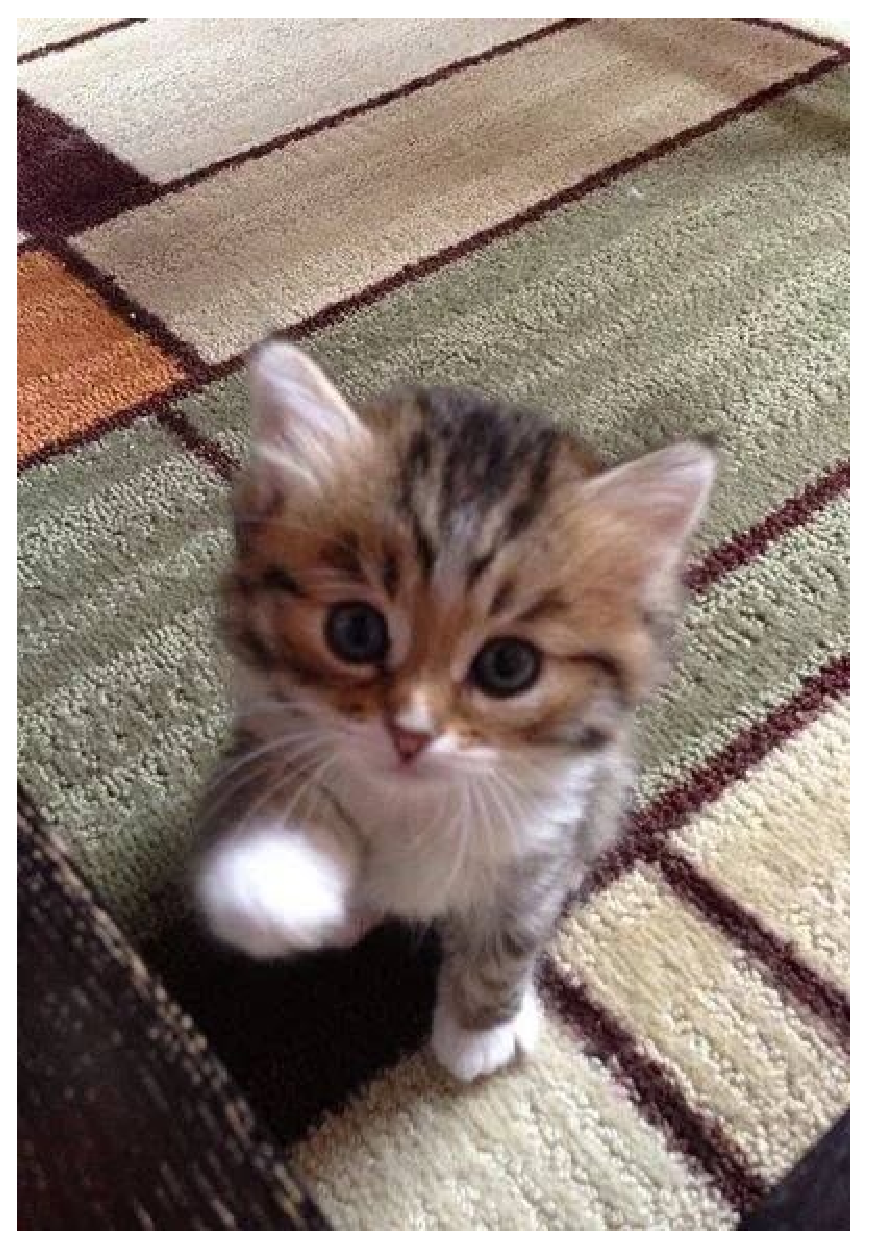
\includegraphics[width=1.5in]{../figures/kitty.eps}
    \end{center}
  \end{frame}

  \begin{frame}{Problem: Scale Variation}
    \begin{center}
      \includegraphics[width=3in]{../figures/kitty_scale_variation.eps}
    \end{center}
  \end{frame}

  \begin{frame}{Problem: Occlusion}
    \begin{center}
      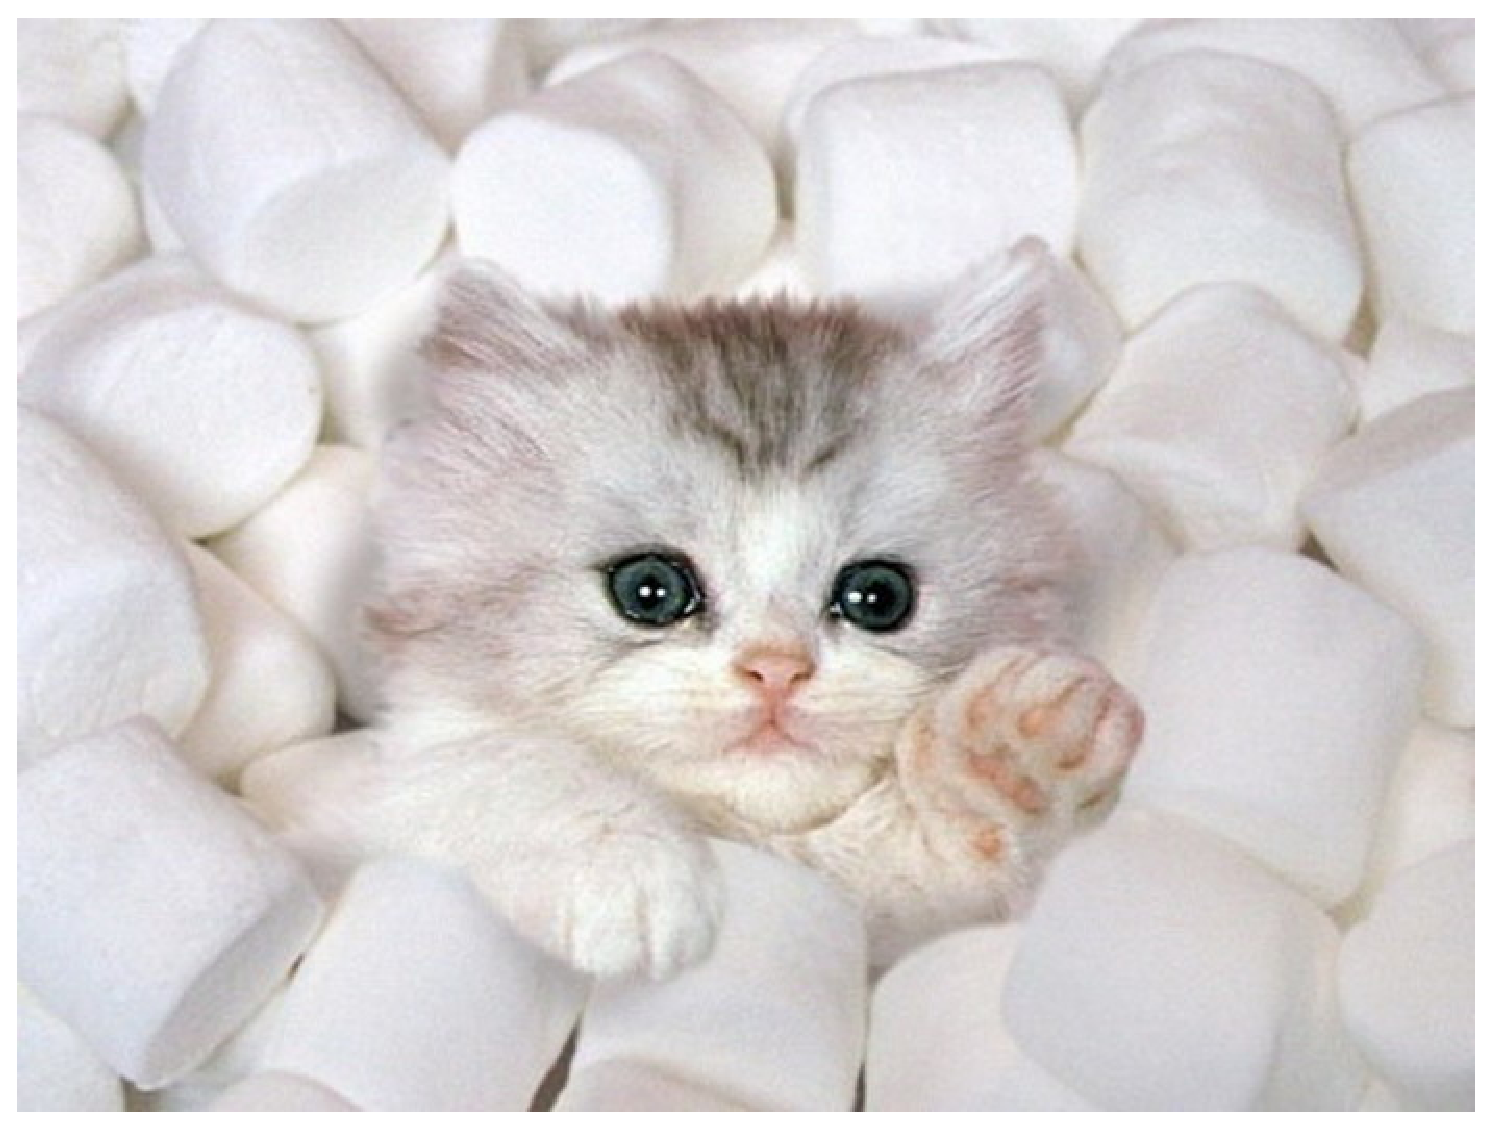
\includegraphics[width=3in]{../figures/kitty_occlusion.eps}
    \end{center}
  \end{frame}

  \begin{frame}{Problem: Deformation}
    \begin{center}
      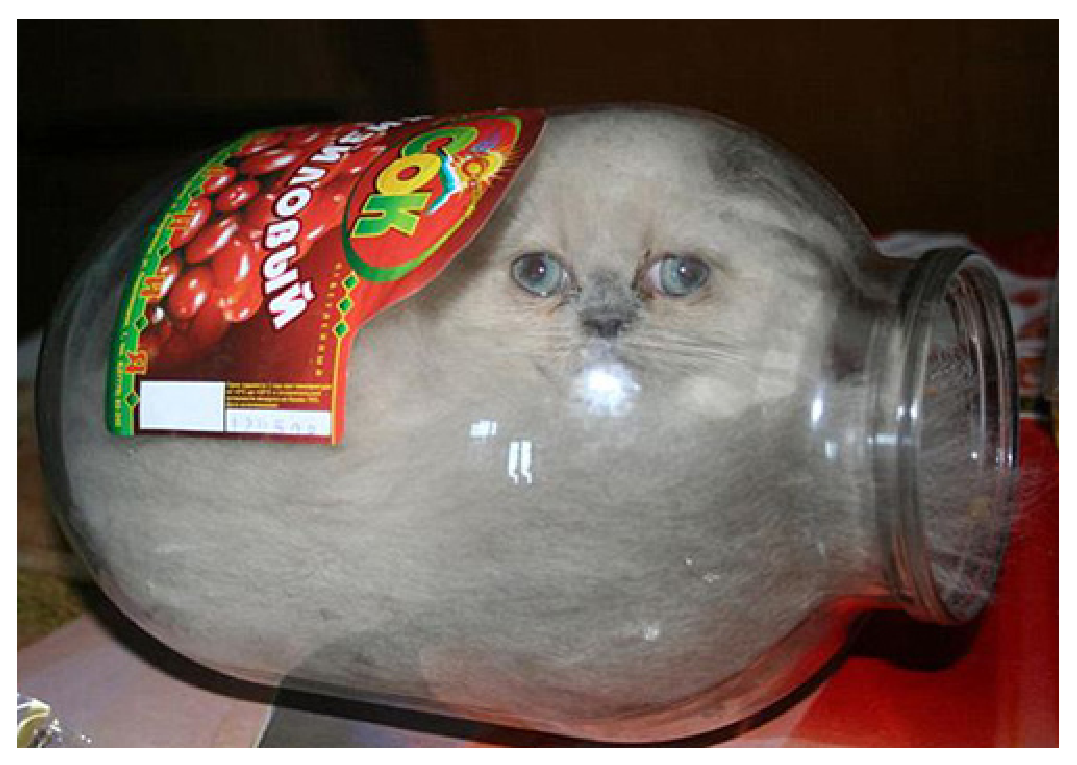
\includegraphics[width=3in]{../figures/cat_deformed.eps}
    \end{center}
  \end{frame}

  \begin{frame}{Problem: Intra-Class Variation}
    \begin{center}
      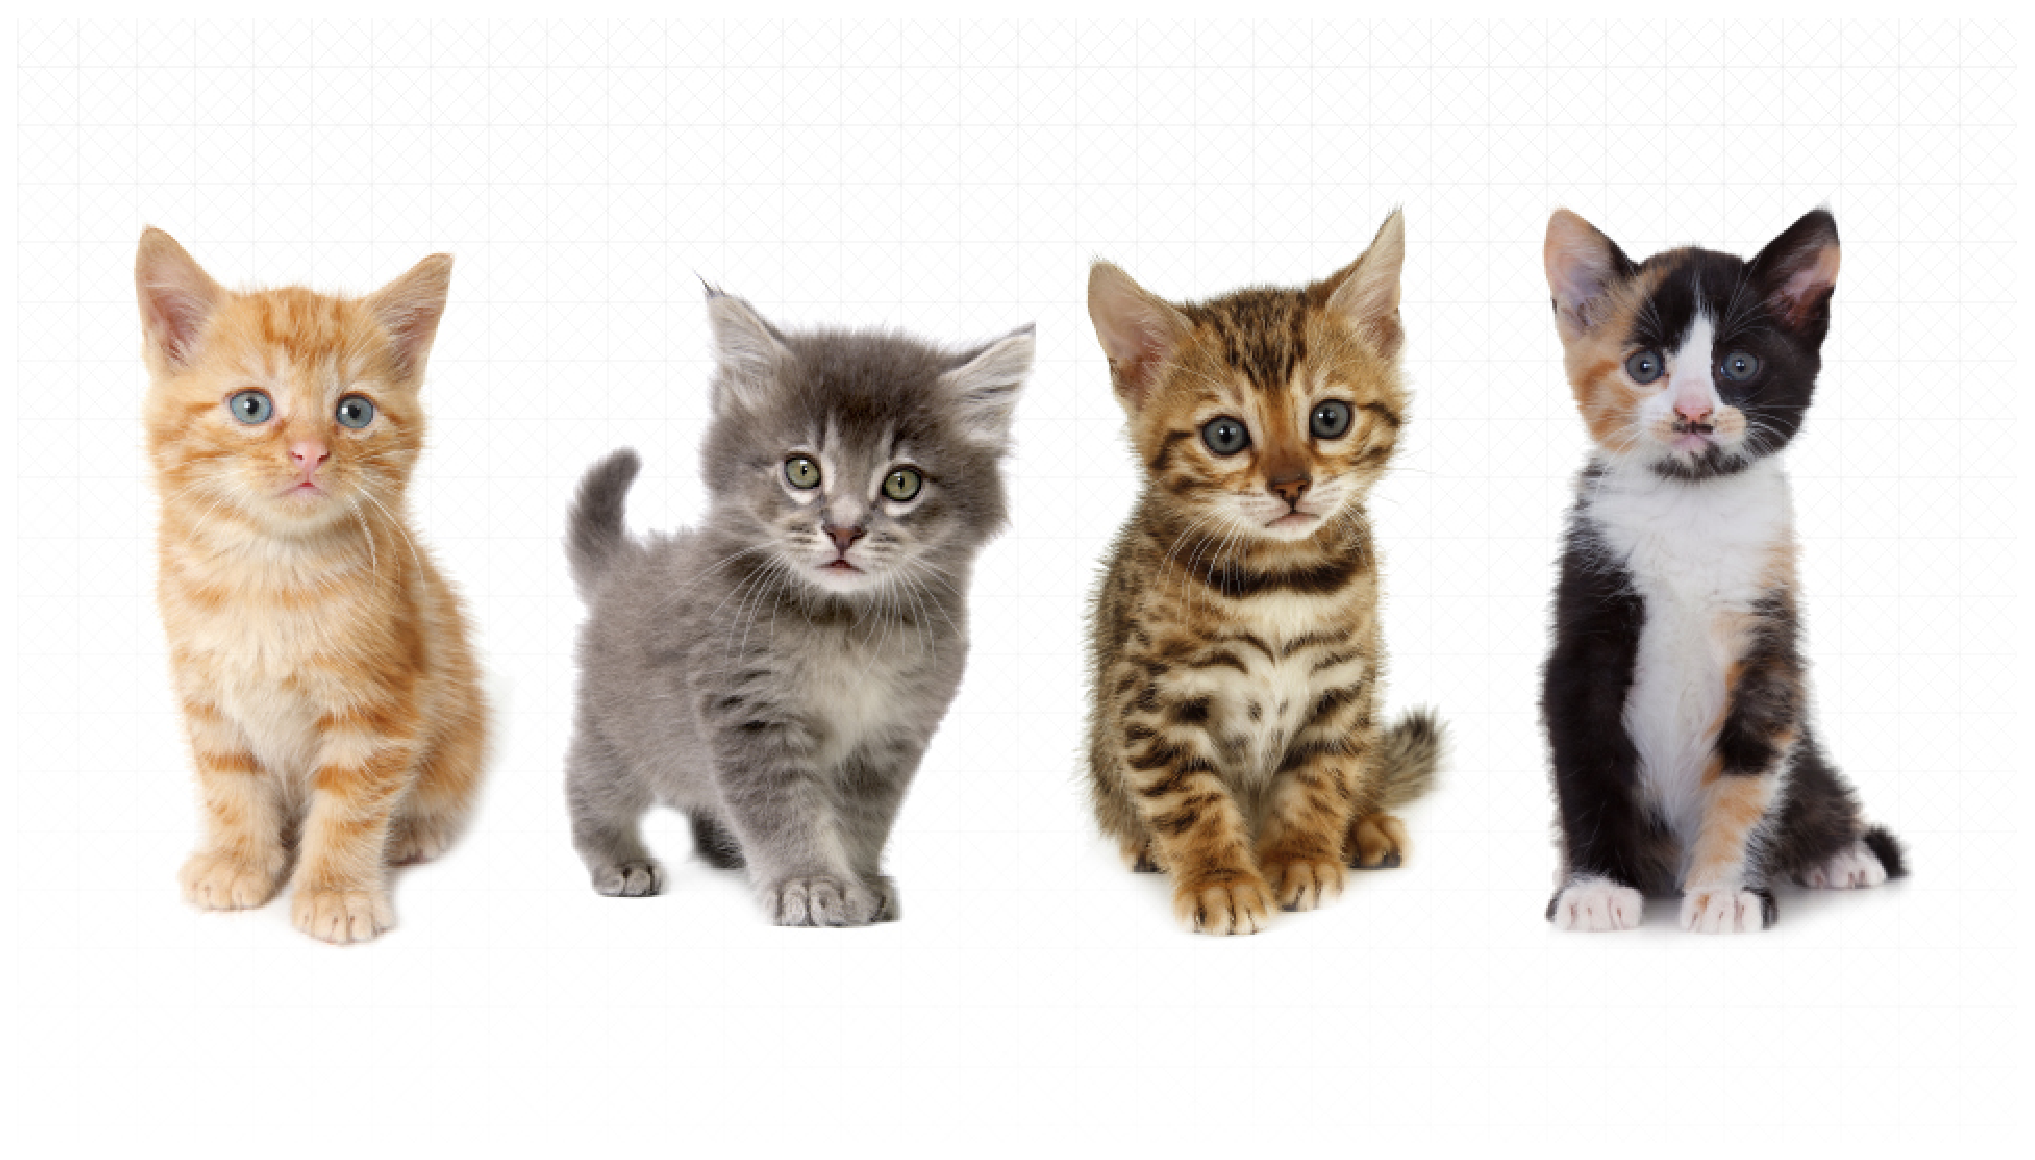
\includegraphics[width=3in]{../figures/kitty_intra_class_variation.eps}
    \end{center}
  \end{frame}

  \begin{frame}{Other Problems}
    \begin{itemize}
      \item images of the same object class are varied
      \item how to generalize to other objects?
      \item Solution: data driven approach
      \begin{itemize}
        \item provide algorithm with many varied examples of each class (i.e. 5000)
      \end{itemize}
    \end{itemize}
  \end{frame}

  \begin{frame}{Why Image Classification?}
    PADs Project
    \begin{itemize}
      \item goal: determine the contents of a pharmaceutical sample
      \item how to process image of a PAD
    \end{itemize}
    \begin{center}
      \includegraphics[width=3in]{../figures/pad.eps}
    \end{center}
  \end{frame}


  \begin{frame}{Datasets: MNIST}
    \begin{itemize}
      \item handwritten digit recognition
      \item 28x28 pixel, greyscale
      \item 50,000 training images, 10,000 testing images
    \end{itemize}
    \begin{center}
      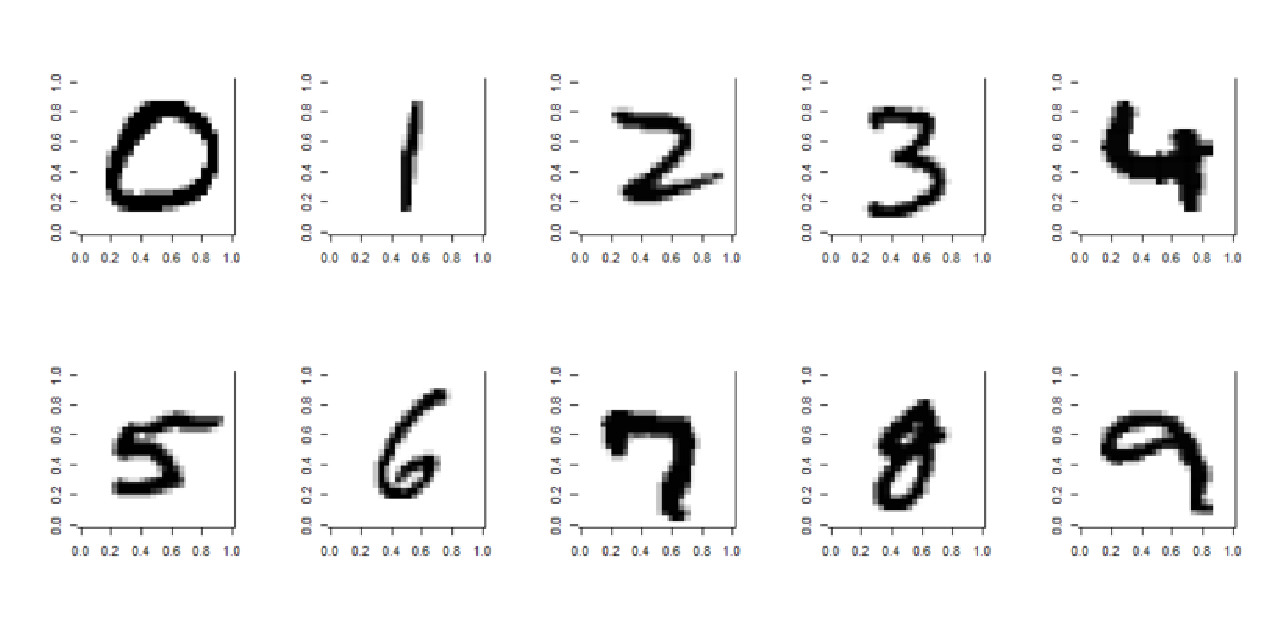
\includegraphics[height=2in]{../figures/mnist.eps}
    \end{center}
  \end{frame}

  \begin{frame}{Datasets: CIFAR10}
    \begin{itemize}
      \item object classification
      \item 32x32 pixel, RGB images
      \item 50,000 training images, 10,000 testing images
    \end{itemize}
    \begin{center}
      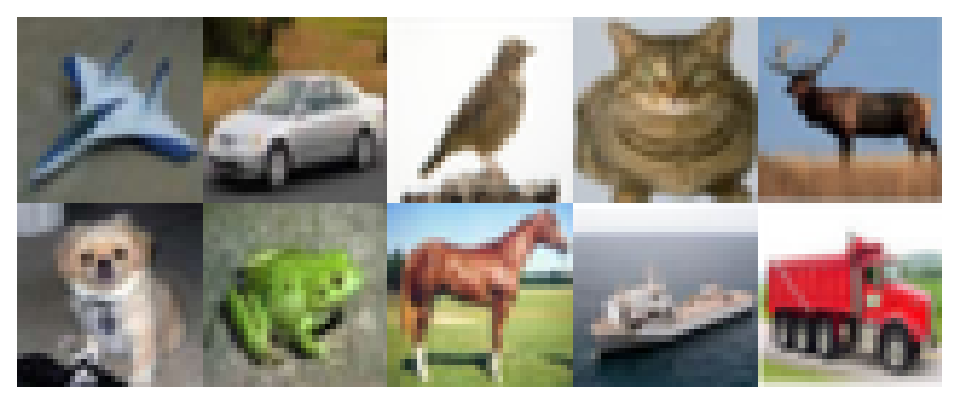
\includegraphics[height=1.5in]{../figures/cifar.eps}
    \end{center}
  \end{frame}

  \section{Workflow}
  \begin{frame}{To Work On}
    \begin{itemize}
      \item gradient descent algorithm
      \item linear classifiers
      \item types of neural networks
      \begin{itemize}
        \item convolutional
        \item deep
        \item recurrent
      \end{itemize}
      \item additional neural network features
      \begin{itemize}
        \item dropout % determines nodes to ignore - prevents overfitting
        \item batch normalization
      \end{itemize}
      \item implementation in Python
    \end{itemize}
  \end{frame}

  \section{Thank-you!}
\end{document}
